\documentclass[letterpaper,12pt,twoside]{uncthesis}

%%%%%%%%%%%%%%%%%%%%%%%%%%%%%%%%%%%%%%%%%%%%%%%%%%%%%%%%%%%%
% Required thesis information
%%%%%%%%%%%%%%%%%%%%%%%%%%%%%%%%%%%%%%%%%%%%%%%%%%%%%%%%%%%%

% When indicating your degree in the second bracketed space, use the full
% degree name (i.e., Doctor of Philosophy, not Ph.D. or PHD; Master of Public
% Health, not M.P.H. or MPH; Master of Social Work, not M.S.W. or MSW).
\uncdegreename{Doctor of Philosophy}

% List your department, school, or curriculum rather than your subject area or
% specialty discipline in the third bracketed space. You may include your
% subject area or specialty discipline in parentheses (i.e., Department of
% Romance Languages (French); School of Pharmacy (Molecular Pharmaceutics);
% School of Education (School Psychology); or similar official area).
% If you wish to include both your department and school names, list the school
% at the end of the statement (i.e., Department of Pharmacology in the School
% of Medicine).
\uncthesisdepartment{Department of Computer Science}

% Type can be dissertation or thesis
\uncthesistype{dissertation}

% Title
\uncthesistitle{Efficient, Locality-Maintaining Namespace Operations in a Write-Optimized File System}

% Name
\uncthesisauthor{Yang Zhan}

% University Name
\uncthesisuniversity{University of North Carolina at Chapel Hill}

% The year in which your committee approves the completed thesis or
% dissertation. This need not be the year you graduate.
\uncthesisyear{2019}

% Thesis advisor. Appears on the abstract page.
\uncthesisadvisor{Donald E. Porter}

% Thesis committee. Appears on the title page.  Do not include titles such as
% Professor, Doctor, Dr., PhD, or any identifiers such as “chair” or “advisor”
% before or after any names.  Put a new line after each name to render
% correctly on title page.
\uncthesiscommittee{Donald E. Porter\\
Leonard McMillan\\
F. Donelson Smith\\
Rob Johnson\\
Ethan L. Miller
}

%%%%%%%%%%%%%%%%%%%%%%%%%%%%%%%%%%%%%%%%%%%%%%%%%%%%%%%%%%%%
% Font selection
%%%%%%%%%%%%%%%%%%%%%%%%%%%%%%%%%%%%%%%%%%%%%%%%%%%%%%%%%%%%
% Font, if using PDFLaTeX
\usepackage{times}
% Font, if using XeLaTeX
%\usepackage{fontspec}
%\setmainfont{Times New Roman}

% Prevent awkward hyphenations.
\hyphenation{Raj-kumar}

\begin{document}
% The following order of the contents is REQUIRED
\pagenumbering{roman}


% 1. Title Page
\newgeometry{left=\uncthesisleftmargin in,top=2in,right=\uncthesisrightmargin in,bottom=1in,nohead}

\begin{titlepage}

\begin{singlespace}
\centering

\currentpdfbookmark{TITLE}{bk:title}

\vspace{1in}
\begin{adjustwidth}{0.5in}{0.5in}
\centering
\MakeUppercase{\uncthesistitle}
\end{adjustwidth}

\nointerlineskip\vspace{1in}

\uncthesisauthor{}

\nointerlineskip\vspace{1in}

\noindent
A \uncthesistype{} submitted to the faculty at the \uncthesisuniversity{} in partial fulfillment of the requirements for the degree of \uncdegreename{} in the \uncthesisdepartment{}.

\nointerlineskip\vspace{1in}

Chapel Hill\\
\uncthesisyear{}
%\the\year

\end{singlespace}

% Use the following block if you want the committee members to have exactly a 1in margin to the right.
%\nointerlineskip\vspace{0.83in}
%\setlength\topsep{0pt}
%\begin{flushright}
%{
%\setlength{\tabcolsep}{0pt}
%\begin{tabular}[t]{l}
%Approved by: \\
%\thesismembers
%\end{tabular}
%} % large
%\end{flushright}

% Use the following block if you want the committee members to appear approximately 2/3 the way across the page.
\nointerlineskip\vspace{0.71in}
\begin{flushright}
\begin{minipage}{2.1in}
\setlength{\tabcolsep}{0em}
\begin{tabular}{l}
Approved by: \\
\uncthesiscommittee{}
\end{tabular}
\end{minipage}
\end{flushright}

\end{titlepage}


% 2. Copyright Page (optional)
%\newgeometry{left=\uncthesisleftmargin in,top=8.42in,right=\uncthesisrightmargin in,bottom=1in,nohead}

\begin{center}
\begin{singlespace}
\copyright~\uncthesisyear\\
\uncthesisauthor \\
ALL RIGHTS RESERVED
\end{singlespace}
\end{center}

\clearpage
\newgeometry{left=\uncthesisleftmargin in,top=2in,right=\uncthesisrightmargin in,bottom=1in,nohead}
% Normal pages from here on out; TOC title takes care of 2in requirement.
\restoregeometry


% 3. Abstract
\begin{abstract}

There seems to be a trade-off between good locality and efficient namespace
operations in file systems.
Traditional inode-based file systems have good rename performance, but fail
to maintain locality, especially in the face of file system aging.
On the other hand, full-path-indexed file systems ensure locality, however,
renaming a directory needs to update all related full-paths,
which is usually implemented as an expensive operation.

This dissertation describes a technique that has both good locality and
efficient namespace operations.
In particular, we describe a novel synthesis of write-optimization,
full-path indexing and operations on data structures.
By directly manipulating the data structure, a full-path-indexed file system
can efficiently update related full-paths in a rename.
Moreover, with the technique, a full-path-indexed file system can
clone a directory without traversing the directory.

We implement this technique in \betrfs, a full-path-indexed, write-optimized,
local file system for Linux.
Compared to ext4, the widely used inode-based file system in Linux,
the new version of \betrfs traverses the Linux source directory 9.47x faster,
and renames the same directory 1.09x faster.
Meanwhile, the new version of \betrfs clones a directory faster than
file systems that clone the directory through file clones,
such as Btrfs and XFS.

\end{abstract}


% 4. Dedication, Acknowledgement(s), Preface (each optional)
%\begin{dedication}
A dedication is a message from the author prefixed to a work in tribute to a person, group, or cause. Most dedications are short statements of tribute beginning with \textit{``To \ldots''} such as \textit{``To my family''}.
\end{dedication}

%\begin{acknowledgement}

Acknowledgements are the author's statement of gratitude to and recognition of the people and institutions that helped the author's research and writing.

    \lipsum[5]
\end{acknowledgement}

%\begin{preface}

A preface is a statement of the author's reasons for undertaking the work and other personal comments that are not directly germane to the materials presented in other sections of the thesis or dissertation. These reasons tend to be of a personal nature.

    \lipsum[6]

\end{preface}


% 5. Table of Contents, with page references
%\renewcommand{\contentsname}{\hfill\bfseries\normalsize TABLE OF CONTENTS\hfill}
%\renewcommand{\cfttoctitlefont}{\hfill\Large\bfseries}
\renewcommand{\cftaftertoctitle}{\hfill}
\renewcommand{\cftdotsep}{1.5}
\cftsetrmarg{1.0in}

\setlength{\cftbeforetoctitleskip}{56pt}
\setlength{\cftaftertoctitleskip}{18pt}

% format chapter entries like other entries
\renewcommand{\cftchapfont}{\normalfont}
\renewcommand{\cftchappagefont}{\normalfont}
\renewcommand{\cftchapleader}{\cftdotfill{\cftdotsep}}

\setlength{\cftbeforechapskip}{15pt}
\setlength{\cftbeforesecskip}{10pt}
\setlength{\cftbeforesubsecskip}{10pt}
\setlength{\cftbeforesubsubsecskip}{10pt}

\begin{singlespace}
\currentpdfbookmark{TABLE OF CONTENTS}{bk:contents}
\tableofcontents
\end{singlespace}

\clearpage


% 6. List of Tables, with titles and page references (if applicable). And list
% of Figures or Illustrations, with titles and page references (if applicable)
%\renewcommand{\listtablename}{LIST OF TABLES}
\phantomsection
\addcontentsline{toc}{chapter}{LIST OF TABLES}

\setlength{\cftbeforelottitleskip}{-14pt}
\setlength{\cftafterlottitleskip}{22pt}
\renewcommand{\cftlottitlefont}{\hfill\normalsize\bfseries}
\renewcommand{\cftafterlottitle}{\hfill}

\setlength{\cftbeforetabskip}{12pt}
\cftsetrmarg{1.0in}

\setlength{\cfttabindent}{0in}

\begin{singlespace}
\listoftables
\end{singlespace}

\clearpage

%\renewcommand{\listfigurename}{LIST OF FIGURES}
\phantomsection
\addcontentsline{toc}{chapter}{LIST OF FIGURES}

\setlength{\cftbeforeloftitleskip}{-14pt}
\setlength{\cftafterloftitleskip}{22pt}
\renewcommand{\cftloftitlefont}{\hfill\normalsize\bfseries}
\renewcommand{\cftafterloftitle}{\hfill}

\setlength{\cftbeforefigskip}{12pt}
\cftsetrmarg{1.0in}

\setlength{\cftfigindent}{0in}

\begin{singlespace}
\listoffigures
\end{singlespace}

\clearpage


% 7. List of Abbreviations (if applicable)
%\phantomsection
\addcontentsline{toc}{chapter}{LIST OF ABBREVIATIONS}

\begin{center}
\textbf{LIST OF ABBREVIATIONS}
\vspace{16pt}
\end{center}

% TODO: define new column types to make sure multi-line table cells has single-spacing

\noindent
\begin{tabular}{p{0.8in} p{5in}}
CoS     & Chamber of Secrets\\
DA      & Dumbledore's Army\\
DADA    & Defence Against the Dark Arts\\
DH      & Deathly Hallows \\
FBAWTFT & Fantastic Beasts and Where to Find Them\\
SPEW    & Society for the Protection of Elvish Welfare\\
VWI     & Voldemort War One\\
VWII    & Voldemort War Two\\
\end{tabular}

\clearpage


% 8. List of Symbols (if applicable)
%\phantomsection{}
\addcontentsline{toc}{chapter}{LIST OF SYMBOLS}

\begin{center}
\textbf{LIST OF SYMBOLS}
\vspace{16pt}
\end{center}

\noindent
\begin{tabular}{@{}p{0.8in} l}
$M$ & Number of wands\\
$m$ & Number of wizards\\
$n$ & Number of fantastic beasts\\
\end{tabular}

\clearpage


\pagenumbering{arabic}

%\chapter{Formatting Guide}
\label{chap:formatting_guide}

\section{Margins}

This template follows the UNC graduate school thesis/dissertation formatting guide as rigidly as possible.
This template has uniform margins throughout the entire document:
\begin{itemize}
    \item Left: 1''
    \item Right: 1''
    \item Top: 1''
    \item Bottom: 1''
\end{itemize}

\section{Font}
A TrueType font is recommended/required by the ProQuest dissertation publishing. Recommended fonts and sizes can be found in \autoref{tab:font}.

\begin{table}
    \centering
    \caption{Recommended font type and size}\label{tab:font}
    \begin{tabular}{ll}
        \toprule
        Font name            & Font Size \\ \midrule
        Arial                & 10pt\\
        Century              & 11pt\\
        Courier New          & 10pt\\
        Garamond             & 12pt\\
        Georgia              & 11pt\\
        Lucida Bright        & 10pt\\
        Microsoft Sans Serif & 10pt\\
        Tahoma               & 10pt\\
        Times New Roman      & 12pt\\
        Trebuchet MS         & 10pt\\
        Verdana              & 10pt\\ \bottomrule
    \end{tabular}
\end{table}

If you're using \texttt{pdflatex} to compile this template, include the \texttt{times} package in the preamble.
If you're using \texttt{xelatex} to compile this template, you can use the \texttt{fontspec} package and the \texttt{setmainfont} command to choose your favorite font.
This template by default uses 12pt Times New Roman.

\section{Spacing and Indentation}

The template takes care of spacing and indentation:
\begin{itemize}
    \item Text appears in a single column on each page and is double-spaced throughout the document.
    \item New paragraphs are indicated by a consistent tab indentation throughout the entire document.
    \item The document text is left-justified.
    \item For blocked quotations, indent the entire text of the quotation consistently from the left margin.
\end{itemize}

\lipsum[6]
\begin{quote}
    This is an example showing the indentation of block quoted text.
    \lipsum[8]
\end{quote}
\lipsum[7]

\section{Pagination}
This template takes care of pagination.

Pagination and margin are also well maintained for landscape pages.
\begin{landscape}
    \lipsum[9] Let's also see how does footnote works in landscape pages~\footnote{We have a footnote in landscape environment}.
\end{landscape}

\section{Footnotes and Endnotes}
Footnotes\footnote{\lipsum[10]} and endnotes\footnote{\lipsum[11]} obey the
formatting guide. However, using both of them confuses the note numbering.
Given the discrepancy between the official format guide\endnote{\lipsum[12]}
and the official sample pages\endnote{\lipsum[14]}, the correct order for
endnotes and appendixes are unclear.  Thus, using only footnote is recommended.

\section{Tables and Figures}
Tables, figures, and illustrations vary widely by discipline. Therefore, formatting of these
components is largely at the discretion of the author.

List of figures and list of tables are well taken care of by \LaTeX{} and this
template.  If an entry in LOT/LOF takes up more than one line, break up the
entry about three-fourths of the way across the page and place the rest of the
text on a second line, single-spacing the two lines.

One nice trick is the short caption option for the
\texttt{\textbackslash{}caption{}} command.  It allows the LOT/LOF only include
the short caption but not the full caption.
\begin{figure}
    \centering
    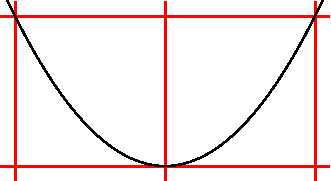
\includegraphics[width=0.5\textwidth]{figures/demo.pdf}
    \caption{A very long caption that does not make much sense but only tests the line-breaking and line-spacing in LOT/LOF.}
\end{figure}

\begin{figure}
    \centering
    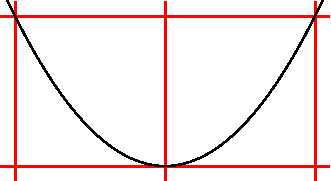
\includegraphics[width=0.5\textwidth]{figures/demo.pdf}
    \caption[Short Caption]{A very long caption that does not make much sense but only tests the line-breaking and line-spacing in LOT/LOF.}
\end{figure}

\section{Reference}
The APA style is used for references. Notice the differences caused by different citation command.

\begin{table}
    \centering
    \caption[Short title]{Comparison of different citation command.}\label{tab:citation}
    \begin{tabular}{ll}
        \toprule
Command                        & Results \\ \midrule
\texttt{\textbackslash{}cite}  & \cite{LFR}\\
\texttt{\textbackslash{}citep} & \citep{LFR}\\
\texttt{\textbackslash{}citet} & \citet{LFR}\\\bottomrule
    \end{tabular}
\end{table}

\section{Length}
There are no requirements for the length of the PhD thesis. For the Department of Computer Science, from 2014 to 2017, average length of the thesis main body text is $\mu \approx 120, \sigma \approx 33$, average length of main body text + reference is $\mu \approx 129, \sigma \approx 35$.
%\chapter{Related Works}
\label{chap:related}

\section{A very long section title testing the line-breaking and line-spacing in TOC if not long enough we make it longer}
\subsection{Subsection title}
\lipsum{}
\subsubsection{Subsubsection title}
\lipsum[1]
\subsection{Another subsection title}

\chapter{Introduction}
\label{chap:intro}

Today's general purpose file systems fail to utilize the full bandwidth of the
underlying hardware.
Widely used inode-based file systems, such as ext4, XFS, and Btrfs, can write
large files at near disk bandwidth,
but typically create small files at less than 3\% of the disk bandwidth.
Similarly, these file systems can read large files at near disk bandwidth,
but scanning directories with many small files is slow, and the performance
degrades when the file system ages~\citep{betrfs3}.

At the heart of this issue is how data is organized on disk.
The most common design pattern for modern file systems is to use multiple layers
of indirection.
The inode number of a file or directory connects the name of an entry in a
directory to its metadata location on disk.
The metadata of an inode contains extents that describes the physical location
and length of data at different offsets.
Indirection simplifies implementation of the file system, and makes some
operations, such creating files and appending files, easy to implement.
In particular, namespace operations are simple and flexible.
For example, a rename is just a pointer swing, moving an entry from one
directory to another directory.
However, indirection doesn't impose any constraint on how metadata and data
are placed on the disk.
In the worst case, the metadata of entries under a directory and the content of
a file can end up scattered over the disk.
Heuristics, such as cylinder groups~\citep{ffs1}, are designed to mitigate this
problem.
However, on modern inode-based file systems, unless the metadata or data are
modified, their location doesn't change.
Therefore, after disk space is allocated and freed over file system aging,
the free space on disk becomes scattered,
leading to bad performance for both reads and writes.

One attempt to solve the problem of random writes is the log-structured file
system~\citep{lfs}.
The log-structure file system treats the disk as a log, so small random writes
becomes log appends, which are significantly faster.
However, the log cleaner in a log-structured file system has severe impact on
performance~\citep{lfsbsd}, especially when the log is full.
And the log-structured file system still uses multiple levels of
indirection, resulting in slow directory traversals.

An alternative design is to use full-path indexing upon write-optimized
dictionaries (WODs) in a file system, known to have good performance on nearly
all operations.
On one hand, WODs have fast random write performance.
A WOD divides its data into multiple levels whose sizes grow exponentially.
Writes are put to the lowest level, and gradually merged to higher levels in
batches.
This merging process in a WOD keeps data sorted in a certain order at each level
and acts as a cleaner to garbage-collect lower levels.
On the other hand, full-path indexing ensures metadata and data in
depth-first-search order, that is, lexicographic order by the full-path names
of files and directories.
With full-path indexing, metadata and data under one directory are close to each
other in key space, which, combined with the sorted order maintained by
WODs, leads to good locality and fast directory traversals.
Prior work~\citep{betrfs1,betrfs1tos,betrfs2,betrfs2tos,betrfs3} of this design
realizes efficient implementation of many file-system operations, such as random
writes, file creates and directory traversals,
but a few operations still have prohibitively high overheads.

The Achilles' heel of such design is the performance of namespace operations,
in particular, renaming large files and directories.
For instance, renaming a large directory changes the full-paths of all files
and directories under it, which updates keys of the metadata and
data and moves them in the key space.
Competitive performance for namespace operations in full-path-indexed file
systems should complete in an I/O-efficient manner.

However, prior work mainly focuses on the schema level of the file system, i.e.,
how metadata and data are keyed and indexed in the WODs.
The full-path-indexed file system usually implements a rename by
fetching all key/value pairs of metadata and data,
inserting them back with updated keys, and deleting old key/value pairs.
Therefore, a rename needs to call several operations for each affected full-path
names, leading to bad performance.
Or, the file system partly backs away from full-path-indexing and adopts
relative-path-indexing, a hybrid of full-path-indexing and indirection.
This approach not only breaks the locality of full-path-indexing, but also
taxes other operations for efficient namespace operations.

This dissertation presents I/O-efficient ways to do namespace operations in a
full-path-indexed, write-optimized file system.
Specifically, though full-path indexing limits possible change on the schema
level, we observe that it can make all full-path names under a directory
contiguous in key space.
And the underlying WOD, \bets, has a tree structure, which makes it possible to
move or clone a contiguous key range efficiently.
Therefore, we dig into the underlying \bets, and implements two new operations,
range-rename and range-clone, that completes file system renames and clones with
bounded number of I/Os.

Chapter~\ref{chap:bg} talks about the necessary background of this dissertation.
We start with a presentation of the write-optimized \bets,
showing the idea of write-optimization.
Then, we describes full-path-indexed \betrfs and relative-path-indexed \betrfs.
The full-path-indexed \betrfs shows the benefit of full-path indexing combined
with write-optimization, but suffers from slow renames.
The relative-path-indexed \betrfs has good rename performance, but breaks the
full-path indexing and taxes other operations for efficient renames.

Chapter~\ref{chap:rename} presents the range-rename operation on \bets,
which full-path-indexed \betrfs can use to implement file system renames.
A range-rename updates all keys with one prefix to another prefix efficiently
through two techniques, \textbf{key lifting} and \textbf{tree surgery}.

Chapter~\ref{chap:clone} expands range-rename to range-clone,
which full-path-indexed \betrfs can use to implement both file or directory
renames and clones.
We first show how to implement range-clone with range-rename techniques by
transforming \bets into \bedags.
Then, we introduces a new type of messages, \goto messages, that works as other
messages in \bedags, fitting range-clone into write-optimization.

Chapter~\ref{chap:eval} evaluates the implementation.
We compare full-path-indexed \betrfs with range-rename or range-clone to
widely used file systems on micro and application benchmarks.
We also put a particular focus on benchmarking the range-rename and range-clone
operations.

Chapter~\ref{chap:related} summarize some previously published work related to
this work.
We organize related work by topic, and talk in detail about work that is closely
related to this work.

Chapter~\ref{chap:conclusion} summarizes and concludes the dissertation.

The primary contribution of this dissertation is to show that there is no
trade-off between efficient namespace operations and locality.
Efficient renames are possible in a full-path-indexed file system, which ensures
locality.
And full-path indexing creates more opportunities for namespace operations,
such as directory clones.



% The graduate school Format Guide put endnotes before appendixes But the
% provided sample pages put appendixes before endnotes It's unclear which one
% is correct. Recommend to use footnotes instead of endnotes.
%\appendix
%\chapter{Example Appendix}
\label{chap:appendix}
\lipsum[1]

\chapter{Another Appendix}
\label{chap:appendix2}

\lipsum[1]

\clearpage

%\begin{center}
\vspace*{46pt}
\currentpdfbookmark{ENDNOTES}{bk:endnotes}
\textbf{ENDNOTES}
\vspace{10pt}
\end{center}
\addcontentsline{toc}{chapter}{ENDNOTES}

\theendnotes{}

\clearpage


\clearpage
\phantomsection

{\def\chapter*#1{} % suppress bibliograph header.
\begin{singlespace}
\addcontentsline{toc}{chapter}{REFERENCES}
\begin{center}
\textbf{REFERENCES}
\vspace{17pt}
\end{center}

\bibliographystyle{apalike}
\bibliography{references}
\end{singlespace}
}


\end{document}
